Voici le document sans la section « Certifications ».

```latex
\documentclass[11pt,a4paper]{article}

\usepackage[T1]{fontenc}
\usepackage[utf8]{inputenc}
\usepackage[british]{babel}
\usepackage[left=0mm,right=0mm,top=0mm,bottom=0mm]{geometry}
\usepackage[stretch=25,shrink=25,tracking=true,letterspace=30]{microtype}
\usepackage{graphicx}
\usepackage{xcolor}
\usepackage{marvosym}
\usepackage{enumitem}
\setlist{parsep=0pt,topsep=0pt,partopsep=1pt,itemsep=1pt,leftmargin=6mm}
\usepackage{FiraSans}
\renewcommand{\familydefault}{\sfdefault}
\definecolor{cvblue}{HTML}{304263}

% --- Macros perso ------------------------------------------------------------
\newcommand{\dates}[1]{\hfill\mbox{\textbf{#1}}}
\newcommand{\is}{\par\vskip.5ex plus .4ex}
\newcommand{\smaller}[1]{{\small$\diamond$\ #1}}
\newcommand{\headleft}[1]{\vspace*{3ex}\textsc{\textbf{#1}}\par%
    \vspace*{-1.5ex}\hrulefill\par\vspace*{0.7ex}}
\newcommand{\headright}[1]{\vspace*{2.5ex}\textsc{\Large\color{cvblue}#1}\par%
     \vspace*{-2ex}{\color{cvblue}\hrulefill}\par}

\usepackage[colorlinks=true,urlcolor=white,linkcolor=white]{hyperref}

% -----------------------------------------------------------------------------

\begin{document}
\setlength{\topskip}{0pt}\setlength{\parindent}{0pt}\setlength{\parskip}{0pt}
\setlength{\fboxsep}{0pt}\pagestyle{empty}\raggedbottom

% ============================================================================
%                               COLONNE GAUCHE
% ============================================================================
\begin{minipage}[t]{0.33\textwidth}
\colorbox{cvblue}{\begin{minipage}[t][5mm][t]{\textwidth}\null\hfill\null\end{minipage}}
\vspace{-.2ex}
\colorbox{cvblue!90}{\color{white}
\kern0.09\textwidth
\begin{minipage}[t][293mm][t]{0.82\textwidth}\raggedright
\vspace*{2.5ex}

% ---- Identité ---------------------------------------------------------------
\Large Pape Saliou \textbf{\textsc{FALL}} \normalsize

\null\hfill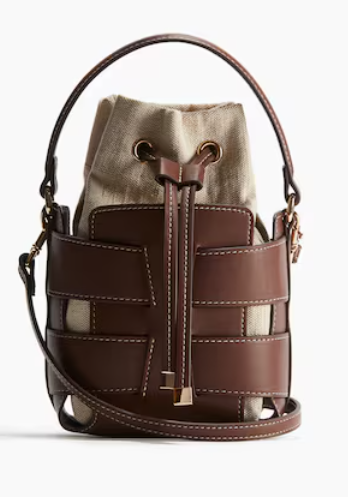
\includegraphics[width=0.65\textwidth]{ 77bf068f9d5a4e33b383d87c34217238.png }\hfill\null

\vspace*{0.5ex}

% ---- Résumé -----------------------------------------------------------------
\headleft{Profile Summary}
Data scientist diplômé de Sorbonne Université, passionné par l’extraction de valeur à partir de grands volumes de données. Solide expérience en modélisation prédictive, en automatisation de pipelines et en visualisation de données pour la prise de décision. Orienté impact business, capable de collaborer avec des équipes pluridisciplinaires et de déployer des solutions data-scalables en production.

% ---- Contact ----------------------------------------------------------------
\headleft{Contact details}\small
\MVAt\ {\small papesalioufall2@gmail.com} \\[0.4ex]
\Mobilefone\ 0753481453 \\[0.5ex]
\Letter\ Paris, Île-de-France, France
\normalsize

% ---- Infos perso ------------------------------------------------------------
\headleft{Personal information}
Citizenship: \textbf{Sénégalaise} \\[0.5ex]
Family: \textbf{Célibataire} \\[0.5ex]
Languages: \textbf{Français, Anglais, Wolof}

% ---- Compétences ------------------------------------------------------------
\headleft{Skills}
\begin{itemize}
  \item Python
  \item R
  \item SQL
  \item Machine Learning
  \item Deep Learning
  \item NLP
  \item Statistics
  \item A/B Testing
  \item Data Visualization (Power BI, Tableau)
  \item Cloud (AWS, GCP)
\end{itemize}

\end{minipage}\kern 0.09\textwidth
}
\end{minipage}
% ============================================================================
%                               COLONNE DROITE
% ============================================================================
\hskip2.5em
\begin{minipage}[t]{0.56\textwidth}
\setlength{\parskip}{0.8ex}
\vspace{2ex}

% ------------------------ EXPÉRIENCE ----------------------------------------
\headright{Experience}
\textsc{Data Scientist} at \textit{Prepaya} (Paris, France)  \dates{2022-09 -- 2023-08} \\
\smaller{Développé des modèles de prédiction de churn utilisant XGBoost, améliorant la rétention de 12 \%}\is
\smaller{Automatisé un pipeline d'extraction et de nettoyage de données avec Python et Airflow, réduisant le temps de traitement de 30 \%}\is
\smaller{Mis en place des dashboards interactifs sous Power BI pour le suivi des KPI produits}\is
\smaller{Collaboré avec des équipes pluridisciplinaires (marketing, produit) pour transformer les insights data en actions business}\is
\smaller{Déployé un modèle de recommandation sur AWS SageMaker, augmentant le panier moyen de 8 \%}\is

% ------------------------ ÉDUCATION ----------------------------------------
\headright{Education}
\textsc{Master 2 Data science}. \textit{Sorbonne Université}. \dates{2022-2023} \\

% ------------------------ HOBBIES -------------------------------------------
\headright{Hobbies}
\textit{Football, Échecs, Voyages}

\end{minipage}

\end{document}